\section{Research Problem}
\label{sec::ResearchProblem}

The research problem addressed in this thesis revolves around the limitations of current robotic systems in dynamic and human-populated environments. While traditional behaviour-based systems provide a structured approach to robot control, they often lack the flexibility to adapt to unpredictable human behaviors. On the other hand, learning-based systems offer adaptability but are heavily dependent on the quality and diversity of their training datasets. This research seeks to explore the integration of generative models, such as LLMs and VLMs, with behaviour-based systems to enhance the robot's ability to respond dynamically to environmental stimuli and human interactions.

\begin{figure}[h]
\centering
\vspace{5mm}
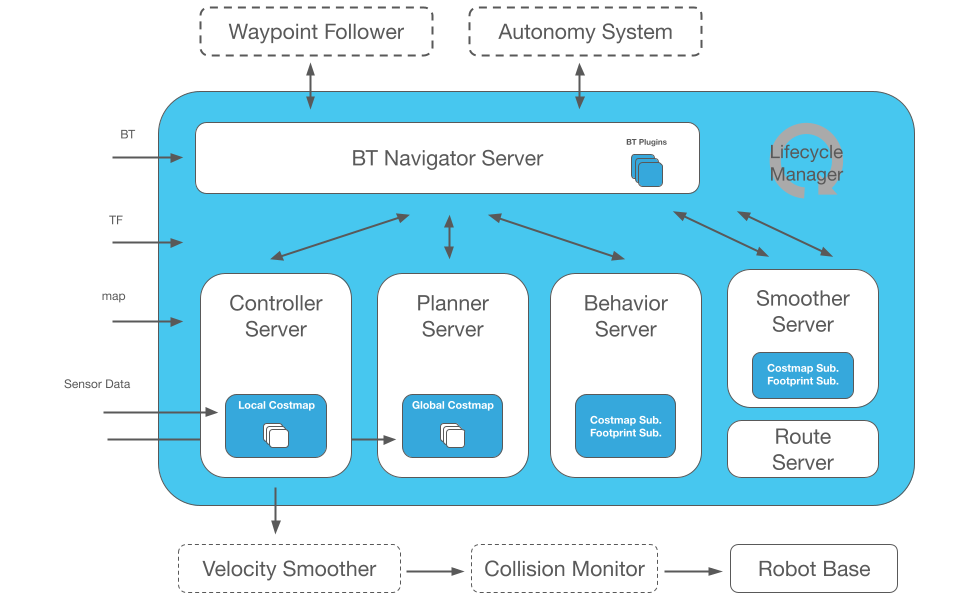
\includegraphics[width=\textwidth]{introduction/figures/nav2_architecture.png}
\caption{Nav2 system architecture from https://docs.nav2.org/}
\label{fig::nv2_strucutre}
\end{figure}

The following research questions have been identified to address these challenges:

\begin{enumerate}
    \item \textit{How can robots exhibit dynamic behaviour in socially aware contexts, and what are the core principles and system requirements necessary to enable effective adaptability?} 
    
    Humans are highly dynamic creatures; thus, when robots are designed to coexist with humans, robots must be capable of dynamically replanning themselves in real time based on changes in the environment, tasks, or human behaviours. In socially aware robotics, this means not just reacting to physical changes but also adapting appropriately to social cues, cultural norms, and contextual expectations. To bring these dynamic replanning capabilities to existing robots and to improve adaptability, the ideal systems need to utilise existing development interfaces and provide a standardised interface themselves.
    
    \item \textit{How can attention be implemented in socially aware robots, and what sensory inputs and guiding principles govern robotic attention mechanisms?}

    To understand when to perform dynamic replanning, robots need to pay attention to the environment and understand what is happening around them. "Attention" in robots is analogous to human attention as it allows a robot to focus on the most relevant environmental stimuli via visual, auditory and proximity sensing. In socially aware settings, attention mechanisms help robots prioritise interaction with people, gestures, speech, or objects based on context, task relevance, and social norms.
    
    \item \textit{What are the key requirements for long-term dynamic task replanning in human-robot interaction, and how does active, interaction-driven planning influence its effectiveness over time?}

    Tasks often evolve in human-robot interaction (HRI). A robot’s initial plan may need to change due to unexpected events, new goals, changes in human behaviour, or changes in the environment. Long-term dynamic replanning enables robots to stay relevant, efficient, and aligned with human needs. When operating long-term, the robots must know and manage their resources, including energy and processing power, and balance autonomy with user interaction.
    
\end{enumerate}
